%%%%%%%%%%%%%%%%%%%%%%%%%%%%%%%%%%%%%%%%%

%----------------------------------------------------------------------------------------
%       Clase, paquetes y configuraciones
%----------------------------------------------------------------------------------------

\documentclass[11pt, a4paper]{article} % Font size

\usepackage[utf8]{inputenc}
\usepackage[T1]{fontenc}
\usepackage[spanish,es-nolayout,es-nodecimaldot,es-tabla]{babel}
\usepackage{amsmath}
\usepackage{amsfonts}
\usepackage{amssymb,amsthm}
\usepackage{enumerate}
\usepackage{enumitem}
\usepackage{parskip}
\usepackage{nicefrac}
\usepackage[left=2cm,right=2cm,top=2.5cm,bottom=2cm]{geometry}
\usepackage[colorlinks = true]{hyperref}
\usepackage{graphicx}

%
\newtheorem{teo}{Teorema}

% Comandos
\newcommand{\R}{\mathbb{R}}
\newcommand{\yds}{\qquad\text{y}\qquad}
\DeclareMathOperator{\proy}{proy}
\DeclareMathOperator{\dd}{d}

\linespread{1.25}

%----------------------------------------------------------------------------------------
%       Datos informativos
%----------------------------------------------------------------------------------------
\title{\begin{large}CURSO DE LATEX\end{large}\\ Tarea 5 Capitulo 6}
\author{Dario Astudillo}
\date{\today}   

% Contenido
\begin{document}
	\maketitle
La solución de la ecuación diferencial
 
	\begin{align*}
	  y^{'}(x)+2y(x)&= \begin{cases}
	1&  \text{si} \quad x \in [0,3], 
	\\
	%x(n), & \text{si} \quad n \leq -1 \\
	0& \text{si} \quad x \textgreater 3 ;     \\	 	
	\end{cases}
	\\ \text{sujeto a}\quad \quad &\\
	 y(0)&=0\\
	\end{align*}
esta dada por la función a trozos 
	\[
	 y(x) = \begin{cases}
	\dfrac{1}{2}(e^{-2x}-1)&  \text{si} \quad x \leq 3,
\\
	 \\    
    \dfrac{1}{2}(e^{-2x}-e^{6-2x})& \text{si}\quad x   \textgreater 3.
	 \\	 	
	\end{cases}
     \]
\begin{center}
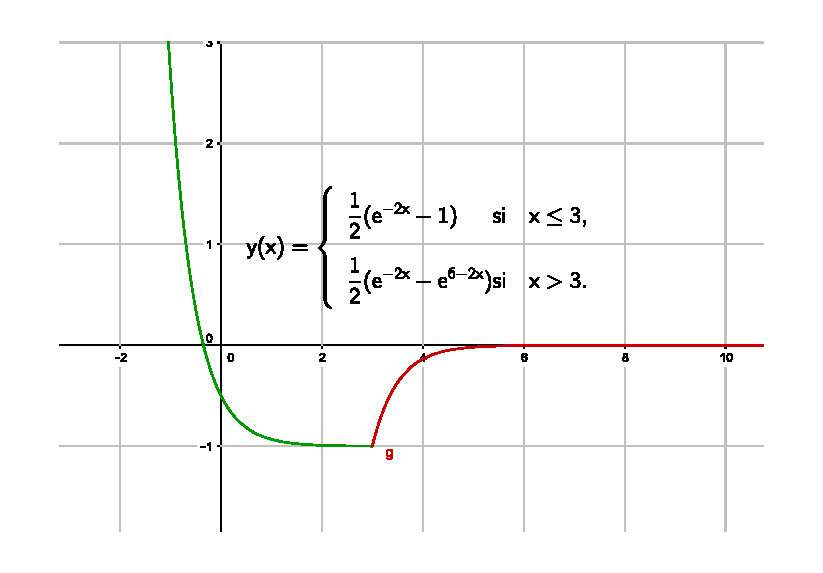
\includegraphics[scale=0.9]{geo1.pdf}
\end{center}
% Table generated by Excel2LaTeX from sheet 'Hoja1'
\begin{table}[htbp]
  \centering
  \caption{Add caption}
    \begin{tabular}{r}
     \\
    \end{tabular}%
  \label{tab:addlabel}%
\end{table}%

\end{document}